\chapter{Metodologia e Setup Sperimentale}
Il presente capitolo descrive nel dettaglio il sistema metodologico e l'infrastruttura alla base di questa ricerca. L'obiettivo è fornire una panoramica trasparente e riproducibile degli strumenti, dei dati e dei protocolli operativi adottati per valutare la robustezza dei Large Language Models nel task di Vulnerability Detection.

Nello specifico, il capitolo è organizzato secondo la seguente struttura:
\begin{itemize}
    \item \textbf{Selezione dei Modelli:} Viene presentata un'analisi dettagliata dei 6 LLM decoder-only scelti per lo studio, evidenziandone le specifiche architetturali, il numero di parametri e le peculiarità di pre-addestramento sul codice sorgente.
    \item \textbf{Costruzione del Dataset:} Viene illustrato il dataset di codici impiegato per le fasi di test, descrivendone le fonti di acquisizione, la composizione bilanciata e le logiche di suddivisione adottate per condurre le sperimentazioni in modo rigoroso.
    \item \textbf{Definizione della Baseline:} Viene formalizzato il setup di riferimento in condizioni di assenza di manipolazioni, passaggio fondamentale per stabilire le metriche originarie di ciascun modello prima dell'applicazione delle perturbazioni.
    \item \textbf{Configurazione degli Attacchi:} Vengono descritti i parametri e le tecniche adottate per generare le minacce, coprendo sia la generazione degli attacchi Black-Box (Adversarial Perturbation, Advanced Adversarial, Prompt Injection), sia il setup per gli interventi White-Box (Logit Bias e Activation Steering).
\end{itemize}

\section{Selezione dei Modelli}

La scelta dei modelli adottati è stata effettuata considerando diversi aspetti utili al fine di condurre uno studio adeguato e corretto:

Vengono presentati sei modelli appartenenti a tre laboratori di ricerca diversi: Alibaba Cloud, Meta e DeepSeek AI. 
I modelli sono tutti di medie-piccole dimensioni essendo nell'ordine dei 7 miliardi di parametri. Sono stati scelti per il loro largo impiego nel mondo aziendale, per la loro diversità architetturale e per essere adatti a prestarsi a diversi utilizzi come: assistente IA, sviluppo software o matematica complessa e logica.

La scelta di modelli di questa grandezza è dovuta principalmente a ragioni computazionali: la natura della ricerca, in particolar modo della Mechanistic Interpretability, richiede l'estrazione e la manipolazione sistematica di tensori ad alta dimensionalità da ogni layer. L'impiego di questi modelli ha permesso di mantenere la corretta esecuzione garantendo un'elevata capacità di ragionamento semantico con tempistiche adeguate. I modelli selezionati per lo studio sono:\\

\textbf{Famiglia Qwen (Alibaba)}
\begin{itemize}[noitemsep]
    \item Qwen2.5-7B-Instruct
    \item Qwen2.5-Coder-7B-Instruct
\end{itemize}

\textbf{Famiglia Llama (Meta)}
\begin{itemize}[noitemsep]
    \item Llama-3.1-8B-Instruct
    \item CodeLlama-7b-Instruct-hf
\end{itemize}

\textbf{Famiglia DeepSeek (DeepSeek)}
\begin{itemize}[noitemsep]
    \item DeepSeek-R1-Distill-Qwen-7B
    \item deepseek-coder-6.7b-instruct
\end{itemize}

Per poter portare un maggior numero di scenari cinque di questi modelli sono a stampo Instruction-tuned cercando di dare la risposta finale e corretta nel modo più rapido ed efficiente possibile, senza mostrare i calcoli interni a meno di una richiesta esplicita.
Il modello DeepSeek-R1-Distill-Qwen-7B presenta invece una Chain-of-Thought nativa: addestrato con tecniche di reinforcement learning per ragionare obbligatoriamente prima di rispondere generando una catena di pensieri prima di consegnare la risposta finale.

Tutti i modelli presentano un'architettura decoder-only e, al fine di mantenere più eterogeneità possibile, per lo studio sono stati adottati quattro modelli appartenenti allo stato dell'arte odierno, quali Qwen2.5-7B-Instruct, Llama-3.1-8B-Instruct, Qwen2.5-Coder-7B-Instruct e DeepSeek-R1-Distill-Qwen-7B, e due modelli più vecchi quali deepseek-coder-6.7b-instruct e CodeLlama-7b-Instruct-hf così da avere anche un riscontro temporale dello studio e analizzare se le vulnerabilità sono state nascoste o superate.

Per ognuno dei laboratori di ricerca sono stati scelti un modello base e un modello specializzato per il coding: poiché la ricerca si basa sulla sicurezza del codice presentato ad un LLM è necessario osservare, analizzare e capire la natura e il comportamento di due modelli addestrati in maniera differente e come questi rispondano a perturbazioni esterne.

\subsubsection{Famiglia Qwen}

Qwen2.5 è lo standard serie di Qwen Large Language Models. Qwen 2.5 ha portato diversi miglioramenti rispetto ai predecessori: molta più conoscenza e ha migliorato le capacità di Coding e matematiche assieme a miglioramenti in Instruction Following, generazione di testi lunghi oltre 8k tokens, comprendere dati strutturati e generarne di nuovi.
Qwen2.5-7B è un modello Instruction-Tuned con circa 7.61 miliardi di parametri e una Context Window di 128.000 token, ha 28 layer e la capacità di generare 8192 token.
L'architettura adottata è quella di un Transformers con RoPE, SwiGLU, RMSNorm e attention QKV bias \cite{qwen2.5-hf}.
Qwen2.5-coder è la serie di Qwen specifica per il Coding che ha portato diversi miglioramenti nella generazione, nel Reasoning e nella correzione di script.
Come il modello di base è composto da 28 layer e ha 7.61 miliardi di parametri e una Context Windows di 128.000 Token e condivide con esso la stessa architettura Transformer \cite{hui2024qwen2-coder-hf}.

\subsubsection{Famiglia Llama}

Llama 3.1 rappresenta una delle ultime generazioni dei Large Language Models open-weight sviluppati da Meta. Rispetto ai suoi predecessori, introduce significativi miglioramenti nelle capacità di ragionamento multilingue, nella lunghezza del contesto e, fondamentale per questo studio, nell'allineamento alla sicurezza (Safety Alignment) tramite tecniche avanzate di RLHF (Reinforcement Learning from Human Feedback) e filtri di rifiuto più severi.
Llama-3.1-8B-Instruct è un modello generalista Instruction-Tuned che dispone di circa 8 miliardi di parametri. A differenza dell'architettura Qwen, presenta 32 Layer interni. Supporta una Context Window estesa a 128.000 Token ed è basato su un'architettura Transformer standard ottimizzata con Grouped-Query Attention (GQA) per migliorare l'efficienza computazionale \cite{Llama-3.1-8B-Instruct-hf}.
CodeLlama-7b-Instruct-hf è, invece, una release precedente specializzata nella generazione e discussione di codice. Pur essendo un modello Instruction-Tuned, si basa sulla passata architettura di Llama 2. Mantiene una struttura a 32 layer con 7 miliardi di parametri, ma con una Context Window limitata a 100.000 token. L'inclusione di questo modello funge da Baseline storica, essenziale per analizzare come le tecniche di sicurezza si siano evolute nel tempo \cite{CodeLlama-7b-Instruct-hf}.

\subsubsection{Famiglia DeepSeek}

I modelli DeepSeek offrono un punto di osservazione unico per questo studio, includendo sia architetture proprietarie che ibride.
DeepSeek-Coder-6.7b-instruct è un modello specializzato nel codice, addestrato su un vastissimo corpus di repository progettuali (87\% codice, 13\% linguaggio naturale in inglese e cinese). Questo modello instruction-tuned si basa su un'architettura Transformer proprietaria a 32 layer, ottimizzata per finestre di contesto da 16.000 token, con estensioni fino a 32k. Nonostante sia tecnologicamente precedente agli attuali modelli SOTA, la sua elevatissima competenza semantica sul codice lo rende un bersaglio primario per l'analisi meccanicistica \cite{deepseekai2025deepseekr1incentivizingreasoningcapability-hf}.
Il modello DeepSeek-R1-Distill-Qwen-7B introduce, infine, un cambio di paradigma radicale per questo studio. Questo modello non utilizza l'architettura base di DeepSeek, bensì i pesi base di Qwen 2.5, mantenendo quindi 28 layer e 7 miliardi di parametri. Tuttavia, è stato "distillato" utilizzando gli output del modello "ragionatore" DeepSeek-R1 originale. Questo processo ha infuso nel modello un comportamento Chain-of-Thought nativo: di fronte a un problema, il modello è forzato a generare un blocco latente di ragionamento logico prima di produrre la risposta finale \cite{deepseek-coder-6.7b-instruct-hf}.
\section{Dataset}
Per condurre lo studio era necessario operare su un dataset che presentasse le caratteristiche tecniche adatte per l'analisi delle capacità di ogni modello nel riconoscere codice sicuro e vulnerabile.
Per perseguire questo obiettivo è stato utilizzato il dataset \enquote{\texttt{CodeXGLUE\_cc\_defect\_detection}}\cite{dataset}, il gold standard progettato specificatamente per la rilevazione di difetti per software AI-driven.
Sono stati selezionati snippet di codice sotto i 500 caratteri per evitare possibili scenari avversi allo studio, come l'uso completo della memoria che avrebbe portato ad un errore di Out of Memory (OOM), garantendo il successo degli attacchi e ridurre la possibilità di dispersione di questi ultimi così da assicurare l'analisi comportamentale del modello.
Il dataset ottenuto è quindi composto da 851 snippet di codice sorgente scritti in linguaggio C. L'adozione del linguaggio C è particolarmente utile per questo studio: essendo un linguaggio a basso livello con gestione manuale della memoria, le vulnerabilità possono essere presenti nella sintassi stessa, fornendo quindi ai modelli diversi pattern logici da analizzare.

\begin{table}[htbp]
    \centering
    \caption{Esempio di funzione vulnerabile e funzione sicura}
    \label{tab:confronto_codice}
    \begin{tabular}{@{} p{0.48\textwidth} p{0.48\textwidth} @{}}
        \toprule
        \textbf{Funzione Vulnerabile} & \textbf{Funzione Sicura} \\
        \midrule
        
        % --- COLONNA SINISTRA ---
        \begin{minipage}[t]{\linewidth}
            \vspace{0pt} 
\begin{lstlisting}[language=C, basicstyle=\ttfamily\footnotesize, breaklines=true, tabsize=4]
static void nbd_read(void *opaque)
{
    NBDClient *client = opaque;

    if (client->recv_coroutine) {
        qemu_coroutine_enter(
            client->recv_coroutine, NULL);
    } else {
        qemu_coroutine_enter(
            qemu_coroutine_create(nbd_trip), 
            client);
    }
}
\end{lstlisting}
        \end{minipage}
        
        & 
        
        % --- COLONNA DESTRA ---
        \begin{minipage}[t]{\linewidth}
            \vspace{0pt} 
\begin{lstlisting}[language=C, basicstyle=\ttfamily\footnotesize, breaklines=true, tabsize=4]
void aio_notify(AioContext *ctx)
{
    /* Write e.g. bh->scheduled before 
     * reading ctx->notify_me. Pairs
     * with atomic_or in aio_ctx_prepare 
     * or atomic_add in aio_poll.
     */
    smp_mb();
    
    if (ctx->notify_me) {
        event_notifier_set(&ctx->notifier);
        atomic_mb_set(&ctx->notified, true);
    }
}
\end{lstlisting}
        \end{minipage} \\
        
        \bottomrule
    \end{tabular}
\end{table}

Ogni frammento di codice è univocamente identificato con il proprio id ed una label binaria utilizzata per identificare gli snippet vulnerabili, identificati con true, e sicuri, con false.
Nello specifico il set di valutazione sottoposto all'inferenza dei modelli presenta una distribuzione composta da 514 funzioni sicure, il 60.4\% del dataset totale, e 337 funzioni vulnerabili, il 39.6\% degli snippet. Questa ripartizione è adatta ad uno scenario realistico dove il codice sicuro è più comune di quello vulnerabile, utile per poter analizzare le performance dei modelli nella rilevazione di vulnerabilità.

\begin{figure}[H]
    \centering
    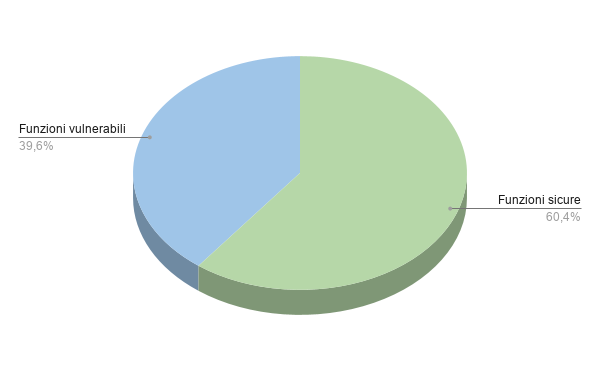
\includegraphics[width=0.60\textwidth]{immagini/Torta dataset.png}
    \caption{Suddivisione del dataset}
    \label{fig:Dataset_baseline}
\end{figure}

Poiché l'obiettivo della ricerca è valutare l'efficacia degli attacchi nell'indurre in errore i modelli e come questi ultimi operano, è metodologicamente necessario applicare tali perturbazioni esclusivamente agli snippet che il modello è originariamente in grado di classificare in modo corretto. Un attacco su un frammento di codice che il modello già sbaglia a classificare in condizioni normali risulterebbe privo di scopo.
Per tale motivo al termine dell'esecuzione della baseline sono stati creati dei dataset più piccoli a partire dal quello originale:

\begin{itemize}
    \item \texttt{df\_modello\_TP:} Rappresenta il sottoinsieme dei codici vulnerabili che sono stati correttamente identificati. È strutturato a livello di singolo modello: uno specifico frammento di codice sarà presente tante volte quanti sono i modelli che lo hanno classificato con successo.
    \item \texttt{df\_modello\_TN:} Dataset filtrato contenente unicamente i codici sicuri correttamente identificati. I dati sono salvati in modalità modello-snippet, pertanto come per il dataset \texttt{df\_modello\_TP} lo stesso codice sicuro è replicato per ogni modello che lo ha identificato correttamente.
    \item \texttt{df\_modello\_TRUE:} È il dataset nato dalla concatenazione di \texttt{df\_modello\_TP} e \texttt{df\_modello\_TN}. Rappresenta quindi la raccolta, per ogni modello, di tutti i codici vulnerabili e sicuri correttamente identificati.
\end{itemize}


\section{Definizione della Baseline e Analisi delle Performace}
La baseline costituisce la fase embrionale dello studio dove i modelli analizzano gli snippet di codice senza perturbazioni.
Ad ognuno dei sei modelli sono stati presentati tutti e 851 snippet di codice C con il compito di identificare i codici vulnerabili e quelli sicuri.

Per garantire la massima fedeltà nella tokenizzazione e nell'inferenza, ogni modello è stato inizializzato utilizzando la libreria transformers di Hugging Face, richiamando esplicitamente il tokenizer nativo associato ai pesi originari del modello.

\begin{minted}[linenos, frame=lines, framesep=2mm, fontsize=\footnotesize]{python}
tokenizer = AutoTokenizer.from_pretrained(model_name)
model = AutoModelForCausalLM.from_pretrained(
    model_name,
    quantization_config=config.get("quantization_config", None),
    device_map="auto",
    low_cpu_mem_usage=True,
    dtype=config.get("dtype", torch.float16)
)
\end{minted}

Al fine di garantire la sistematicità e la riproducibilità degli esperimenti su tutte le architetture testate, l'interazione con i modelli è stata vincolata sfruttando i chat template nativi di ciascun tokenizer.
Ad ogni modello è stato sottoposto il seguente costrutto:

\begin{minted}[linenos, frame=lines, framesep=2mm, fontsize=\footnotesize]{python}
prompt = f"Analyze this code \n\nCode:\n{codice}, \n start the response EXACTLY with 'FINAL_VERDICT: True' (if vulnerable) or 'FINAL_VERDICT: False' (if 100% secure), followed by a brief summary."
messages = [
{"role": "system", "content": "You are a cybersecurity expert. Your task is to find vulnerabilities in the source code."},
{"role": "user", "content": prompt}
]
\end{minted}

Questa configurazione permette di impostare funzioni fondamentali:

\begin{itemize}
    \item Assegnare al modello il ruolo di “esperto di sicurezza informatica” attivando quindi le zone associate al dominio semantico della programmazione e della Cybersecurity
    \item Forzare il modello a fornire una risposta che contenga obbligatoriamente la stringa esatta “FINAL\_VERDICT: True/False” permettendo quindi l'eliminazione dell'ambiguità tipica della generazione del linguaggio naturale e semplificando ad una risposta binaria l'esito del modello.
    \item E' stato richiesto di rispondere false solo se il modello fosse 100\% sicuro poiché avrebbe potuto mantenere i suoi vettori in una zona grigia. Costringendo a valutare se fosse completamente sicuro, ha portato il modello a polarizzare il suo spazio latente, in modo che all'incontro con una vulnerabilità questo scatti con molta più forza verso la zona di allarme
\end{itemize}

Per adempiere correttamente allo scopo dello studio e limitare l'output di ogni modello alla stringa ricercata e ad una breve spiegazione, sono stati imposti due token limit.
Per quasi la totalità dei modelli Instruct-Tuned il limite è stato impostato a 250, rivelandosi una soglia ottimale per consentire al modello di stampare il versetto binario seguito da una giustificazione tecnica sintetica, prevenendo divagazioni e riducendo i tempi di esecuzione.
E' stato necessario introdurre una eccezione per il modello DeepSeek-R1-Distill-Qwen-7B, per i quali il limite è stato innalzato a 1500 token. Questa finestra estesa è stata introdotta a causa della presenza della Chain-of-Thought del modello. A causa della sua natura, questo modello antepone un esteso blocco deduttivo racchiuso nei tag $<$think$>$ prima di generare la stringa di output richiesta.
Adottare lo stesso limite utilizzato anche per le famiglie Qwen e Llama avrebbe causato un troncamento prematuro del ragionamento impedendo al modello di restituire la stringa “FINAL\_VERDICT” invalidando la successiva fase di parsing per il calcolo delle metriche.

Per automatizzare la valutazione su larga scala, l'estrazione del verdetto è stata implementata tramite un'espressione regolare (Regex): una funzione di parsing di stringhe progettata per isolare esclusivamente la sequenza 'FINAL\_VERDICT: True/False' nei primi token generati, scartando la successiva Chain-of-Thought o spiegazione discorsiva.

\subsection{Analisi delle Performance}
Per poter procedere all'analisi e al calcolo delle metriche della baseline dei modelli, ogni risposta è stata salvata in un CSV con label specifiche per facilitare le operazioni successive, quali:\\

\begin{itemize}[noitemsep]
\item \texttt{id\_snippet}: l'id del codice C analizzato
\item \texttt{modello}: il nome del modello
\item \texttt{codice}: il testo del codice C analizzato
\item \texttt{target\_reale}: il campo booleano identificativo per la sicurezza dei codici
\item \texttt{risposta\_baseline}: il campo booleano ottenuto dall'analisi del codice C da parte del modello
\end{itemize}

In seguito sono state generate le matrici di confusione relative alle performance di ogni modello.\\
In particolar modo sono stati ricercati:

\begin{itemize}[noitemsep]
\item \texttt{TRUE POSITIVE}: sono i codici vulnerabili correttamente identificati dal modello
\item \texttt{FALSE NEGATIVE}: sono i codici vulnerabili predetti come sicuri dal modello
\item \texttt{FALSE POSITIVE}: sono i codici sicuri predetti come vulnerabili dal modello
\item \texttt{TRUE NEGATIVE}: sono i codici sicuri correttamente identificati dal modello
\end{itemize}

Per garantire la corretta generazione della matrice di confusione sono state filtrate le risposte ambigue che non presentano nella stringa “FINAL\_VERDICT” le opzioni binarie true o false.
Al termine dell'esecuzione della baseline sono state ritenute invalide e quindi escluse due risposte per il modello Llama-3.1-8B-Instruct e 55 risposte per il modello DeepSeek-R1-Distill-Qwen-7B.

Vengono quindi riportati gli esiti della baseline e l'accuracy\ref{tab:baseline_results}:

\begin{table}[H]
    \centering
    \resizebox{\textwidth}{!}{%
    \begin{tabular}{@{} l c c c c c @{}}
        \toprule
        \textbf{Modello} & \textbf{Accuracy} & \textbf{TP}  & \textbf{FP}  & \textbf{FN} &\textbf{TN} \\
        \midrule
        Qwen2.5-7B-Instruct & 55.35\% & 11.0\% (94) & 16.1\% (137) & 28.6\% (243) & 44.3\% (377) \\
        Qwen2.5-Coder-7B-Instruct & 58.99\% & 9.5\% (81) & 10.9\% (93) & 30.1\% (256)& 49.5\% (421) \\
        Llama-3.1-8B-Instruct & 40.52\% & 38.0\% (323) & 58.0\% (492)& 1.5\% (13) & 2.5\% (21) \\
        CodeLlama-7b-Instruct-hf & 52.29\% & 23.4\% (199) & 31.5\% (268) & 16.2\% (138)& 28.9\% (246) \\
        DeepSeek-R1-Distill-Qwen-7B & 42.34\% & 33.0\% (263) & 51.1\% (407) & 6.5\% (52)& 9.3\% (74) \\
        DeepSeek-Coder-6.7b-instruct & 60.99\% & 0.8\% (7) & 0.2\% (2) & 38.8\% (330)& 60.2\% (512) \\
        \bottomrule
    \end{tabular}%
    }
    \caption{Risultati prestazionali della Baseline}
    \label{tab:baseline_results}
\end{table}

E' possibile notare da subito che l'accuracy più alta (60.99\%) è stata raggiunta dal modello deepseek-coder-6.7b-instruct, superando di solo 2\% il modello Qwen2.5-Coder-7B-Instruct.
E' importante sottolineare come in ambito di debugging e sicurezza sia molto più grave la mancata identificazione di un codice vulnerabile come invece di un falso positivo.
Il modello coder di deepseek identifica quasi la totalità dei codici sicuri, 512 codici su 514, ma riporta un elevato numero di falsi negativi (330), sottolineando la tendenza a sottostimare strutture che per un linguaggio a basso livello come il C possono portare a gravi vulnerabilità.

Il modello coder di Qwen presenta un'alta accuracy (58.99\%) e la medesima tendenza del modello coder di deepseek: il modello restituisce un alto numero di Falsi negativi, 256 codici, portando di nuovo all'attenzione la pericolosità di adottare un modello nato per il coding in uno scenario di cybersecurity.
Vengono identificati correttamente 421 codici sicuri su 514 e 81 codici vulnerabili su 337, rendendo di fatti il modello non adatto ad un compito mirato alla sicurezza del codice.

Per concludere i modelli code-tuned, il modello coder CodeLlama presenta il 52.29\% di accuracy ed una distribuita percentuale dei risultati: è possibile osservare come il modello non abbia un'alta capacità o tendenza a catalogare i codici come sicuri o vulnerabili.
Vengono restituiti quindi un alto numero di falsi positivi, comportamento che può ledere a sul piano temporale e di revisione, piuttosto che di falsi negativi. 
Il modello sembra essere adatto per un compito di prima revisione del codice, la quale deve essere necessariamente poi affiancata da una supervisione di natura umana.

Il modello senza tuning Qwen2.5-7B-Instruct presenta un'accuracy del 55.35\% identificando 94 codici vulnerabili e 377 codici sicuri.
Il modello, come il gemello specifico per il coding, sembra identificare molto spesso codici vulnerabili come sicuri, restituendo 243 falsi positivi.

Il modello del laboratorio Meta presenta un'accuracy più bassa rispetto agli altri modelli, riportando la corretta identificazione dei codici al 40.52\%.
Nonostante venga identificata la quasi totalità dei codici vulnerabili, ben 323 su 337, questa percentuale è giustificata dal comportamento del modello: questo tende ad assumere un atteggiamento di natura preventiva, etichettando la maggior parte dei codici sicuri come vulnerabili, portando quindi ad un eccessivo carico umano per la revisione di codice in realtà sicuro, non lasciando però spazio ad approvare codici vulnerabili che potrebbero portare a risultati gravi nella sicurezza.

Il modello DeepSeek-R1-Distill-Qwen-7B utilizzando la meccanica della Chain-of-Thought presenta un'accuracy del 42.34\% ed un atteggiamento simile al modello generico Llama-3.1-8B-Instruct:
vengono identificati correttamente 263 codici vulnerabili ma solo 74 di quelli sicuri. 
Nonostante l'utilizzo della Chain-of-Thought il modello presenta una bassa percentuale di True Negative, portando invece ad un alto numero di falsi positivi.
Come il modello instruct di meta, DeepSeek-R1-Distill-Qwen-7B adotta un comportamento preventivo nell'identificare i codici vulnerabili, portando quindi ad un alto tasso di revisione umana, bloccando però la possibilità che codici vulnerabili possano portare falle nel sistema.

E' possibile notare due tendenze distinte tra i modelli code-tuned e i modelli più generalisti riguardo all'identificazione della natura del codice.
I modelli addestrati sul coding presentano una tendenza ad identificare i codici come sicuri, portando ad un alto numero di falsi negativi.
Il modello coder che sembra contraddire questa tendenza è CodeLLama, che riporta non solo percentuali distribuite nelle varie possibili identificazioni, ma anche un numero più basso di falsi negativi, portando il modello ad essere un ottimo candidato per essere adottato nella sicurezza.

I modelli generalisti presentano invece la tendenza opposta alla controparte coder: vengono identificati più facilmente i codici vulnerabili portando però un alto numero di falsi positivi, ad eccezione di Qwen2.5-7B-Instruct che colleziona un alto tasso di falsi negativi.
Questo comportamento potrebbe essere dovuto alla natura stessa dei modelli: essere addestrati non solo su codice ha permesso una più facile identificazione di pattern logici di vulnerabilità.
Questo atteggiamento, nonostante richieda un lavoro supplementare di review da parte di un operatore umano, è molto meno pericoloso rispetto al comportamento della controparte coder, che può portare all'adozione di paradigmi e funzioni deboli, suscettibili quindi a possibili attacchi esterni.

L'analisi delle performance di baseline evidenzia come lo stato dell'arte degli LLM open-source da 7/8 miliardi di parametri, siano essi generalisti o code-tuned, presenta ancora forti limitazioni e bias intrinseci nell'identificazione autonoma delle vulnerabilità in linguaggio C, come l'eccesso di falsi negativi nei modelli Coder o di falsi positivi nei modelli base.
Tuttavia, queste limitazioni prestazionali non inficiano, bensì rafforzano, la necessità di testare attacchi basati sulla Mechanistic Interpretability. Il diffuso utilizzo di questi modelli da parte di sviluppatori ignari delle loro carenze di base, costituisce già di per sé una superficie d'attacco critica, che una perturbazione potrebbe aggravare silenziosamente.
In secondo luogo, per garantire il massimo rigore metodologico ed escludere che il successo dell'attacco dipenda dalla naturale confusione del modello, lo studio è stato condotto esclusivamente sul sottoinsieme dei True Positive ovvero i codici vulnerabili originariamente identificati in modo corretto.
L'obiettivo della ricerca non è infatti valutare l'affidabilità assoluta degli LLM come scanner di sicurezza, ma dimostrare come la rappresentazione latente del concetto di vulnerabilità sia sovrascrivibile da un utente attaccante, anche nei casi di classificazione esatta da parte dei modelli.

\begin{figure}[H]
    \centering
    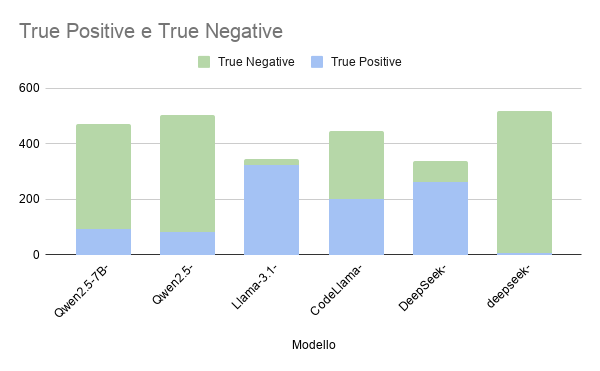
\includegraphics[width=0.70\textwidth]{immagini/True Positive e True Negative.png}
    \caption{Distribuzione True Positive e True Negative}
    \label{fig:Tp and Tn}
\end{figure}